\label{chapter:metodo}
Este Capítulo descreve o método proposto neste trabalho, baseado em VHDL para analise de circuitos utilizando transformações de código e a ferramenta ESBMC.

%======================
%Visão geral do método
%======================
\section{Visão geral do método}
O método consiste na análise de código VHDL de um circuito lógico através de transformação de código e da ferramenta ESBMC. O método consiste inicialmente em um circuito lógico descrito em VHDL, onde assertiva serão inseridas de modo automatizado ou pelo próprio usuário. Este código posteriomente é traduzido para linguagem C e recebe uma instrumentação de código para a posterior analise do mesmo. O Código em C, já instrumentado, será processado e analisado de acordo com as assertivas inseridas e ao final apresenta o resultado positivo ou negativo, caso alguma das assertivas seja violada. Todo o método é apresentado na \autoref{fig:Fluxo_ferramenta} e nas sessões a seguir serão apresentados cada etapa do método proposto neste trabalho

\begin{figure}[H]
	\begin{center}
    \caption{\label{fig:Fluxo_ferramenta}Ciclo da ferramenta}
	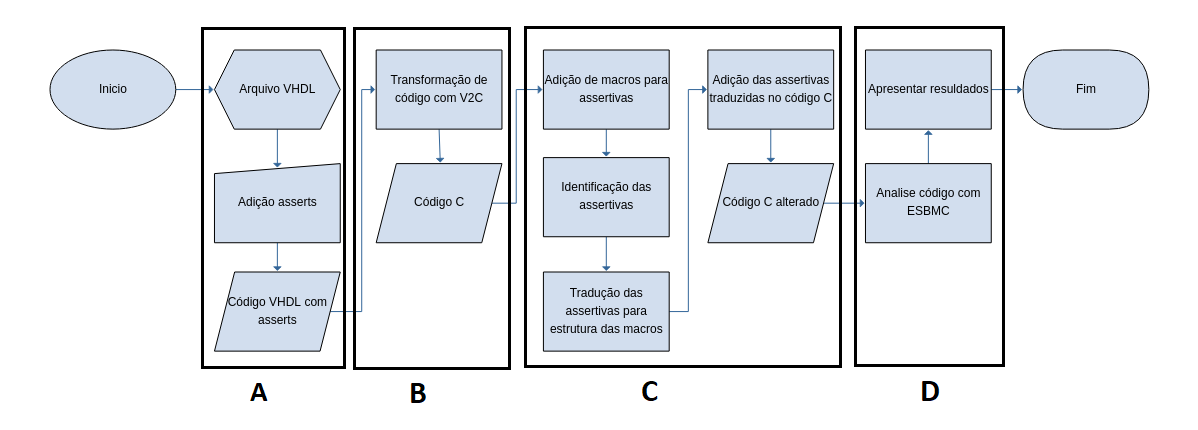
\includegraphics[scale=0.5]{Figuras/Fluxo_ferramenta.png}
	\end{center}
    \legend{Fonte: Própria}
\end{figure}

Com o intuito de auxiliar nas explicações apresentadas nas próximas sessões, o código na \autoref{fig:code_exemplo} será utilizado nas explanações, bem como será apresentado todas as alterações do mesmo, conforme cada etapa do método.
\begin{figure}[H]
\caption{\label{fig:code_exemplo} Exemplo de código VHDL de ULA com portas AND,OR e XOR.}
	\begin{center}
    \begin{minipage}{0.6\textwidth}
    \begin{lstlisting}       
library ieee;
use ieee.std_logic_1164.all;

ENTITY Ula_tcc IS
PORT(A,B,Binvertido,Op1,Op2:IN BIT;
	  Resultado:OUT BIT);
END Ula_tcc;

ARCHITECTURE Ula_tcc_behavl OF Ula_tcc IS
SIGNAL and_port: bit;
SIGNAL or_port: bit;
SIGNAL xor_port:bit;
SIGNAL mux2x1: bit;
BEGIN
	PROCESS(A,B,Binvertido,Op1)
	BEGIN
		--PORTA AND
		IF(A = '1' and mux2x1 = '0') THEN
		    and_port <= '1';
		ELSE
		    and_port <= '0';
		END IF;
		--PORTA OR
		IF(A = '0' and mux2x1 = '0') THEN
		    and_port <= '0';
		ELSE
		    and_port <= '1';
		END IF;
		--PORTA XOR
		IF(A = '0' and mux2x1 = '0') THEN
		    xor_port <= '0';
		ELSIF(A = '1' and mux2x1 = '1') THEN
		    xor_port <= '0';
		ELSE
		    xor_port <= '1';
		END IF;
		--INVERSOR
		IF(Binvertido = '0') THEN
			mux2x1 <= B;
		ELSE
			mux2x1 <= NOT B;
		END IF;
		--MUX4X1
		IF(Op1 = '0' and Op2 = '0') THEN
			Resultado <= and_port;
		ELSIF(Op1 = '0' and Op2 = '1') THEN
			Resultado <= or_port;
		ELSIF(Op1 = '1' and Op2 = '0') THEN
			Resultado <= xor_port;
		END IF;
	END PROCESS;
END Ula_tcc_behavl;
    \end{lstlisting}
    \end{minipage}
	\end{center}
    \legend{Fonte: Própria.}
\end{figure}

%========================
%Código VHDL e assertivas
%========================
\pagebreak
\section{\label{cap:vhdl_assertivas}Código VHDL e assertivas}

\par
A fase inicial do método consiste na adequação do método e inserção das assertivas, conforme a \autoref{fig:Fluxo_ferramenta}, na \textbf{etapa A}. A ferramenta não realiza qualquer tipo de verificação sobre o código VHDL, apenas utiliza o mesmo como entrada juntamente com as assertivas inseridas. Toda verificação é realizada sobre o código em linguagem C, traduzido do código VHDL de entrada.
\par
A adição das assertivas pode ser realizada de maneira automatizada ou manual inserida pelo desenvolvedor de hardware, caso necessite realizar uma verificação mais especifica sobre o código. Mesmo a linguagem VHDL tendo modelo de assertivas padrão, para o método tornou-se necessário a criação de um modelo para que as funções do analisador fossem suportadas.

\par
\label{sec:assertiva_descricao} As assertivas manuais são adicionadas entre as tags \textbf{@c2vhdl:ASSERT} e \textbf{@c2vhdl:END} e todo trecho de código entre estas tags deve estar comentado, desta forma não apresentará erro na tradução do código em linguagem C. As assertivas apresentam as funções necessárias para a análise utilizando a ferramenta ESBMC. A assertiva apresenta três informações principais, sendo elas: condição, mensagem e gravidade.

\begin{figure}[H]
\caption{\label{fig:assertiva} Exemplo de assertiva para verificação de porta XOR.}
	\begin{center}
    \begin{minipage}{0.99\textwidth}
    \begin{lstlisting}       
--@c2vhdl:ASSERT
--assert (Resultado = '1')
--report "O resutado foi diferente de 0"
--severity ERROR;
--@c2vhdl:END
    \end{lstlisting}
    \end{minipage}
	\end{center}
    \legend{Fonte: Própria.}
\end{figure}

\par
A condição representa a assertiva propriamente dita e que será analisado pela aplicação. A condição será precedida de \textbf{--assert} e seguido ou não da palavra \textbf{not}, com isso a assertiva pode assumir valor negativo, conforme necessidade do usuário. Na \autoref{fig:assertiva} a assertiva busca verificar se a variavél Resultado terá igual a 1. 

\par
A mensagem é definida pelo usuário e será apresentado caso a assertiva apresente falha. E precedida pela palavra \textbf{--report}. A severidade pode ser definida como \textit{error}, que representa um erro fatal e parada da verificação e \textit{warning} que representa um erro não fatal, onde é comtabilizado o erro, porém não causa a parada da verificação. É precedido pela palavra \textbf{severity}.

\par
Na \autoref{fig:assertiva} a mensagem a ser exibida em caso de erro é "O resultado foi diferente de 0" e a severidade definida como \textit{error} indicando que é uma assertiva fatal. Na atual implementação da ferramenta não foram utilizadas, sendo a próxima etapa do processo, onde será utilizado um framework para teste de unidade.

\par
Outra propriedade utilizada juntamente com as assertivas é a função \textit{\_\_ESBMC\_assume()}. Esta função utilizada em conjuto com a ferramenta ESBMC permite que durante a verificação uma variavél possa ter uma valor setado durante o tempo de execução da verificação. A importância desta função é fazer verificações onde se conhece os valores de entrada juntamente com o valor resultante, por exemplo, na verificação de portas lógicas.

\begin{figure}[H]
\caption{\label{fig:assertiva} Exemplo de utilização da função \_\_ESBMC\_assume().}
	\begin{center}
    \begin{minipage}{0.99\textwidth}
    \begin{lstlisting}       
    --__ESBMC_assume(A = '1')
    --__ESBMC_assume(mux2x1 = '0');
    \end{lstlisting}
    \end{minipage}
	\end{center}
    \legend{Fonte: Própria.}
\end{figure}

\par
A assertivas automáticas são geradas baseados nas entradas do código VHDL. Seja no modelo manual ou automático, as entradas são mapeadas para serem utilizados na etapa de instrumentação. Desta forma, tais entradas podem ser utilizadas para gerar essas assertivas e então serem adicionadas diretamente ao código em linguagem C durante a fase de instrumentação. 

\par
A \autoref{fig:code_exemplo_assertiva} apresenta o código juntamente com as assertivas conforme o padrão salientado na \autoref{sec:assertiva_descricao}. Neste exemplo foi implementado utilizado a inserção manual das assertivas e também da função \_\_ESBMC\_assume(), entretanto o objetivo é automátizar estas funções durante a execução da ferramenta.
\begin{figure}[h]
\caption{\label{fig:code_exemplo_assertiva} Código da \autoref{fig:code_exemplo} com a assertiva da \autoref{fig:assertiva}.}
	\begin{center}
    \begin{minipage}{0.99\textwidth}
    \begin{lstlisting}       
library ieee;
use ieee.std_logic_1164.all;
...
ARCHITECTURE Ula_tcc_behavl OF Ula_tcc IS
SIGNAL and_port: bit;
SIGNAL or_port: bit;
SIGNAL xor_port:bit;
SIGNAL mux2x1: bit;
BEGIN
	PROCESS(A,B,Binvertido,Op1) IS
	BEGIN
		--PORTA AND
		IF(A = '1' and mux2x1 = '0') THEN
    --__ESBMC_assume(A = '1')
    --__ESBMC_assume(mux2x1 = '0');
		    and_port <= '1';
		ELSE
		    and_port <= '0';
		END IF;
		...
		--MUX4X1
		IF(Op1 = '0' and Op2 = '0') THEN
			Resultado <= and_port;
		ELSIF(Op1 = '0' and Op2 = '1') THEN
			Resultado <= or_port;
		ELSIF(Op1 = '1' and Op2 = '0') THEN
			Resultado <= xor_port;
        --@c2vhdl:ASSERT
        --assert (Resultado = '1');
        --report "O resutado foi diferente de 0";
        --severity ERROR;
        --@c2vhdl:END
		END IF;
	END PROCESS;
END Ula_tcc_behavl;
    \end{lstlisting}
    \end{minipage}
	\end{center}
    \legend{Fonte: Própria.}
\end{figure}

%===================================
%Tradução para código em linguagem C
%===================================
\section{\label{cap:traducao}Tradução para código em linguagem C}
\todo[inline]{Procurar bibtex do do artigo da ferramenta e adicionar ao texto as referencias.}
\par
A etapa seguinte é a tradução deste código para linguagem C, conforme apresentado na \autoref{fig:Fluxo_ferramenta}, \textbf{etapa B}. A partir deste ponto, a ferramenta é executada de maneira propriamente dita, tendo todo o processo automátizado até a apresentação do resultado. Para este método foi selecionado a ferramenta V2C que realiza a tradução de VHDL para Linguagem C.

\par
Devido ser uma ferramenta antiga, a ferramenta V2C apresenta certas limitação na tradução do código VHDL, em outras palavras, a mesma não reconhece algumas estruturas especificas do VHDL. A ferramenta aceita apenas entradas e saídas do tipo: bit, std\_ulogic, qsim\_state, std\_ulogic\_vector e interger. Na parte de arquitetura, a ferramenta aceita uma gama maior de estruturas, trabalhando com expressoões do tipo: signal, variable, integers, strings e caracteres. Em expreções condicionais os operandos são AND, OR, NOT <=, =>,=,<,> e <>. Aceita também a estrutura de process, além da estutura block. A estrutura \textit{process} é limitada apenas a: if-else, case e  loops.
\begin{figure}[h]
\caption{\label{fig:code_traduzido} Código da \autoref{fig:code_exemplo} traduzido pela ferramenta V2C.}
	\begin{center}
    \begin{minipage}{0.99\textwidth}
    \begin{lstlisting}       
void ula_tcc(int in_data[], int out_data[])
{
int _i_=0;
int _cont_;
enum segnale {A, B, Binvertido, Op1, Op2, Resultado, and_port, or_port, 
              xor_port, mux2x1, _MAX_};
int old[_MAX_];
int new[_MAX_];
int chg[_MAX_];
new[A] = (in_data[0]>>_i_) & 0X01; _i_+=1;
new[B] = (in_data[0]>>_i_) & 0X01; _i_+=1;
new[Binvertido] = (in_data[0]>>_i_) & 0X01; _i_+=1;
new[Op1] = (in_data[0]>>_i_) & 0X01; _i_+=1;
new[Op2] = (in_data[0]>>_i_) & 0X01; _i_+=1;
new[Resultado] = (in_data[0]>>_i_) & 0X01; _i_+=1;
new[and_port] = (in_data[0]>>_i_) & 0X01; _i_+=1;
new[or_port] = (in_data[0]>>_i_) & 0X01; _i_+=1;
new[xor_port] = (in_data[0]>>_i_) & 0X01; _i_+=1;
new[mux2x1] = (in_data[0]>>_i_) & 0X01; _i_+=1;

for (_i_=0; _i_<_MAX_; _i_++)
    {
       old[_i_]=new[_i_];
    }
new[A] = in_data[1];
new[B] = in_data[2];
new[Binvertido] = in_data[3];
new[Op1] = in_data[4];
new[Op2] = in_data[5];

for (_i_=0; _i_<_MAX_; _i_++)
    {
    chg[_i_]=old[_i_] ^ new[_i_];
    old[_i_]=new[_i_];
    }

do {
   _cont_=0;
   /* Start of Translation */

   /* p0: */
   if (chg[A] || chg[B] || chg[Binvertido] || chg[Op1]) {
            /*PORTA AND */
      if ((old[A]==1 && old[mux2x1]==0)) {
	   \\__ESBMC_assume(old[A] = 1);
           \\__ESBMC_assume(old[mux2x1] = 0);
         new[and_port]=1;
         }
      else {
         new[and_port]=0;
         }
      /*PORTA OR */
      if ((old[A]==0 && old[mux2x1]==0)) {
         new[and_port]=0;
         }
      else {
         new[and_port]=1;
         }
      /*PORTA XOR */
      if ((old[A]==0 && old[mux2x1]==0)) {
         new[xor_port]=0;
         }
      else if ((old[A]==1 && old[mux2x1]==1)) {
         new[xor_port]=0;
         }
      else {
         new[xor_port]=1;
         }
      /*INVERSOR */
      if ((old[Binvertido]==0)) {
         if (chg[B]) {
            new[mux2x1]=old[B];
            }
         }
      else {
         if (chg[B]) {
            new[mux2x1]=~old[B];
            }
         }
      /*MUX4X1 */
      if ((old[Op1]==0 && old[Op2]==0)) {
         if (chg[and_port]) {
            new[Resultado]=old[and_port];
	    \\@c2vhdl:ASSERT
            \\assert (Resultado = '1');
            \\report "O resutado foi diferente de 0";
            \\severity ERROR;
            \\@c2vhdl:END
            }
         }
      else if ((old[Op1]==0 && old[Op2]==1)) {
         if (chg[or_port]) {
            new[Resultado]=old[or_port];
            }
         }
      else if ((old[Op1]==1 && old[Op2]==0)) {
         if (chg[xor_port]) {
            new[Resultado]=old[xor_port];
            }
         }
      }

   /* End of Translation */
   for (_i_=0; _i_<_MAX_; _i_++)
       {
       if (new[_i_]!=old[_i_]) _cont_=1;
       chg[_i_]=old[_i_] ^ new[_i_];
       old[_i_]=new[_i_];
       }
   } while (_cont_);

new[A] &= 0X01;
new[B] &= 0X01;
new[Binvertido] &= 0X01;
new[Op1] &= 0X01;
new[Op2] &= 0X01;
new[Resultado] &= 0X01;
new[and_port] &= 0X01;
new[or_port] &= 0X01;
new[xor_port] &= 0X01;
new[mux2x1] &= 0X01;

out_data[0]=0; _i_=0;
out_data[0] |= new[A] << _i_; _i_+=1;
out_data[0] |= new[B] << _i_; _i_+=1;
out_data[0] |= new[Binvertido] << _i_; _i_+=1;
out_data[0] |= new[Op1] << _i_; _i_+=1;
out_data[0] |= new[Op2] << _i_; _i_+=1;
out_data[0] |= new[Resultado] << _i_; _i_+=1;
out_data[0] |= new[and_port] << _i_; _i_+=1;
out_data[0] |= new[or_port] << _i_; _i_+=1;
out_data[0] |= new[xor_port] << _i_; _i_+=1;
out_data[0] |= new[mux2x1] << _i_; _i_+=1;

out_data[1] = new[Resultado];
}
    \end{lstlisting}
    \end{minipage}
	\end{center}
    \legend{Fonte: Própria.}
\end{figure}

\par
Na tradução é necessário substituir os operadores originais por seus equivalentes em linguagem C. A excessão são os operadore específicos que geranciam os valores de bit, tai como concatenação ou manipulação de partes verotiais, para os quais são necessários construir procedimentos especificos em C.

Conforme mostrado na \autoref{fig:code_traduzido}, na tradução é verificado a existencia de vários vetores, sendo eles \textbf{chg[]}, \textbf{old[]} e \textbf{new[]}. O vetor \textbf{old[]} contém o valor do sinais do passo anterior e a partir deste vetor o valor a ser usado nos cálculo é obtido. O vetor \textbf{new[]} representa os novos valores a serem calculados pelos antigos e o vetor \textbf{chg[]} contém um or exclusivo entre o valor novo e antigo e em caso de alteração entre os valores é copiado o valor de \textbf{new[]} para \textbf{old[]}.

\par
Os vetores in\_data [] e out\_data [] contêm os sinais de entrada e saída, respectivamente. No caso de circuitos seqüenciais, o valor do status é inserido primeiro (índice 0). a função então lerá os valores in\_data [] e escreverá os resultados do processamento em out\_data []. Ao final da operações os valores de estado são passado para out\_data[].
\par
Conforme especificado e seguindo os parametros da ferramenta, a mesma realiza a tradução, mantendo inalterado qualquer fragmento de código que esteja comentado, neste caso, as assertivas presentes no código VHDL permanecem inalteradas, sendo utilizadas na próxima etapa do processo.

%========================
%Instrumentação de código
%========================
\section{Instrumentação de código}

\par
As assertivas após a tradução permanecem em comentadas, sendo necessário prepara-lás para verificação posterior do código. Com isso é necessário uma instrumentação do código para que o mesmo esteja pronto para análise, conforme apresentado na \autoref{fig:Fluxo_ferramenta}, \textbf{etapa C}.

\par
Todas as etapas da instrumentação são realizados sobre o código já traduzido. O passo inicial da instrumentação é a adição da macros no inicio do código C com as definição das assertivas a serem utilizadas. Na \autoref{fig:macro} apresenta as macros utilizadas no código. A linha 1 corresponde a mensagem de erro a ser apresentada e a linha 2 corresponde ao modelo da assertiva e a chamanda da macro definida na linha 1 em caso de falha. 

\begin{figure}[H]
\caption{\label{fig:macro} Macros das assertivas implementadas em linguagem C}
	\begin{center}
    \begin{minipage}{0.99\textwidth}
    \begin{lstlisting}       
#define log_error(M,...)fprintf(stderr,M,__FILE__,__LINE__,##__VA_ARGS__)
#define __MY_assert(A, M,...) if(!(A)) {log_error(M, ##__VA_ARGS__); assert(A); }
    \end{lstlisting}
    \end{minipage}
	\end{center}
    \legend{Fonte: Própria.}
\end{figure}

\par
O passo seguinte é a identificação das assertivas comentadas ao longo do corpo do texto, utilizando o exemplo da \autoref{fig:assert_c}. As assertivas são identificadas através das tags \textbf{@c2vhdl:ASSERT} e \textbf{@c2vhdl:END} e a busca é realizado através destas tags. Ao ser encontrado a tag \textbf{@c2vhdl:ASSERT}, é realizado um loop até que seja encontrada a tag \textbf{@c2vhdl:END} e com isso toda a assertiva inserida possa ser passada a função de busca das informações da assertiva.

\par
Com a assertiva passada para a função de busca, é realizado a busca da condição, mensagem e severidade através das tags \textbf{--assert}, \textbf{--report} e \textbf{--severity} respectivamente. Esta informações são encontradas através do uso e uma Regex no código e que são adicionadas ao código C seguindo o modelo definido na macro. Este processo é repetido até outra assertiva ser encontrada ou caso chegue ao fina do código C.

\par
Com a função \textit{\_\_ESBMC\_assume()} ocorre processo semelhante ao das assertivas. Utilizando novaente uma regex é realizado a busca por esta função no código e é retirado o comentário da mesma, desta forma a mesma passa a esta acessivél para o ESBMC, visto que a declaração da mesma já segue o modelo padrão a ser utilizado pelo ESBMC.

\par
Durante a instrumentação de código também é realizado a entrada de sisnais não deterministicos, utilizando a função \_\_VERIFIER\_nondet\_int(). Esta função é utilizada em todas as variaveis de entrada e também nos sinais criados ao longo da arquitetura. Desta forma, todas as variavéis necessárias são inicializadas para verificação.
\begin{figure}[htp]
\caption{\label{fig:assert_c} Código com assertivas traduzida para linguagem C}
	\begin{center}
    \begin{minipage}{0.99\textwidth}
    \begin{lstlisting}       
#include<stdio.h>
#define log_error(M, ...) fprintf(stderr,  M , __FILE__, __LINE__, ##__VA_ARGS__)//Update to print the trace
#define __MY_assert(A, M, ...) if(!(A)) {log_error(M, ##__VA_ARGS__); assert(A); }

...

do {
   _cont_=0;
   /* Start of Translation */
    chg[A] = __VERIFIER_nondet_int(); 
    chg[B] = __VERIFIER_nondet_int(); 
    chg[Binvertido] = __VERIFIER_nondet_int(); 
    chg[Op1] = __VERIFIER_nondet_int();
    chg[and_port] = __VERIFIER_nondet_int();
    chg[Resultado] = __VERIFIER_nondet_int();
    chg[or_port] = __VERIFIER_nondet_int();
    chg[mux2x1] = __VERIFIER_nondet_int();

   /* p0: */
   if (chg[A] || chg[B] || chg[Binvertido] || chg[Op1]) {
            /*PORTA AND */
      if ((old[A]==1 && old[mux2x1]==0)) {
	   __ESBMC_assume(old[A] = 1);
           __ESBMC_assume(old[mux2x1] = 0);
         new[and_port]=1;
         }
      else {
         new[and_port]=0;
         }

      ...

      /*MUX4X1 */
      if ((old[Op1]==0 && old[Op2]==0)) {
         if (chg[and_port]) {
            new[Resultado]=old[and_port];
	    __MY_assert(new[Resultado] == 1,"O resultado é diferente de 0");
         }
      else if ((old[Op1]==0 && old[Op2]==1)) {
         if (chg[or_port]) {
            new[Resultado]=old[or_port];
            }
         }
      else if ((old[Op1]==1 && old[Op2]==0)) {
         if (chg[xor_port]) {
            new[Resultado]=old[xor_port];
            }
         }
      }

   /* End of Translation */
...
    \end{lstlisting}
    \end{minipage}
	\end{center}
    \legend{Fonte: Própria.}
\end{figure}

\par
Em outras palavras, na instrumentação de código é realizado a traduçao das assertivas do modelo utilizado no código VHDL para para o modelo utilizado em linguagem C, além como de outras funções que possam ser utilizados pelo VHDL. Ao final da instrumentação fica disponivél o código C para que possa ser entrada para outras ferramentas e não apenas o ESBMC.

%=============================================
%Verificação de assertvas usando model checker
%=============================================
\section{Verificação de assertivas usando \textit{Model Checker}}
\par
O \textit{Model checking} adotado no desenvolvimento de método é o ESBMC na versão 3.0.0 e conforme explicado na \autoref{cap:bounded}, esta ferramenta possui como entrada um código C ou C++ e devido a isso foi escolhida neste projeto. Nesta sessão será apresentado a etapa D da \autoref{fig:Fluxo_ferramenta}.

\par
Para a verificação, a primeira etapa é a busca das assertivas pela ferramenta, para isso é utilizado uma função e através desta a busca das claims, mais especificamente as claims que possuem assertivas, cada claim é identificada através de uma numeração de acordo com a ordem de busca do código analisado. Cada claim com assertivas encontrada é adicionada a uma lista para que seja realizada uma análise individual de cada claim como assertiva.

\begin{figure}[H]
\caption{\label{fig:codigo_claims} Código apresentando a função de busca das clains com assertivas.}
	\begin{center}
    \begin{minipage}{0.99\textwidth}
    \begin{lstlisting}       
VAR
  contador: inteiro
  claim: lista
  claim_string: string 

FUNCAO call_esbmc: arquivo
  contador<-0
  INICIO
  saida<-funcao de geracao das claims pelo ESBMC
  ENQUANTO contador < saida FACA
    contador+=2
    regex para procurar claim e numeracao da claim
    SE encontrar claim ENTAO
      regex para procurar a palavra "assertion"
      SE encontrar a palavra "assention" ENTAO
        contador+=1
	      Adiciona a numeracao da claim na lista
      FIM-SE
    FIM-SE
  FIM-ENQUANTO
FIM-FUNCAO
    \end{lstlisting}
    \end{minipage}
	\end{center}
    \legend{Fonte: Própria.}
\end{figure}

\par
A função apresenta a chamada da ferramenta ESBMC que ocorre na linha 9 da \autoref{fig:codigo_claims} e através da opção \textit{--show-claims} lista todas as claims presentes no texto, como apresentado na \autoref{fig:claims_assertivas}. Juntamente com a opção \textit{--show-claims} é utilizado as opções:
\begin{itemize}
    \item \textbf{--no-pointer-check:} Onde não realiza a checagem de ponteiros no código;
    \item \textbf{--no-div-by-zero-check:} Onde não realiza a checagem de divisões por zero no código.
    \item \textbf{--no-bounds-check:} Onde não realiza a checagem de array bounds no código.
\end{itemize}
Com estas opções o número de claims geradas é reduzida e desta forma gerando um benificio ao programa, que realiza uma quantidade menor de checagem das claims. Com resultado gerado pelo ESBMC é realizado um busca pelas claims com assertivas e gerado uma lista com apenas com estas claims, para posterior análise individual delas.
\begin{figure}[H]
	\begin{center}
    \caption{\label{fig:claims_assertivas}Imagem de claims contendo assertivas.}
	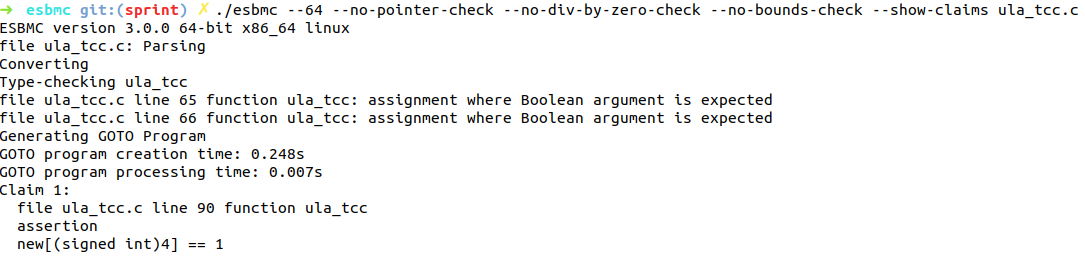
\includegraphics[scale=0.55 ]{Figuras/lista_claim.png}
	\end{center}
    \legend{Fonte:Própria}
\end{figure}
\par
Após a lista das claims com assetivas ser gerada, outra função, indicada na \autoref{fig:analise_claims}, é chamada para verificação de cada claim individualmente. Para cada claim, ocorre a chamada do ESBMC, utilizando as opções \textit{--no-pointer-check}, \textit{--no-div-by-zero-check} e \textit{--no-bounds-check}, juntamente com a opção \textit{--unwind} em que realiza o número de desdobramentos indicado nesta flag. 

\par
Contudo, dependendo da complexidade da assertiva, faz-se necessário aumentar o número de desdobramentos que, por padrão, serão dez. A função é chamada na linha 11 da \autoref{fig:analise_claims} e após a analise da claim é realizado a busca do resultado e exibição caso seja uma propriedade violada.

\par
Desta forma o ESBMC realiza apenas a checagem necessária dentro da assertiva, evitando que outros parametros sejam verificados, sem a devida necessidade do mesmo. Ao final de todos os desdobramentos é apresentado o resultado,apresentado na \autoref{fig:resultado}, sendo positiva ou negativa, dependendo da assertiva e do código analisado. Este processo se repete até a lista de claims contendo assertiva ser finalizada.
\begin{figure}[H]
\caption{\label{fig:analise_claims}Pseudocódigo da função de análise das claims.}
	\begin{center}
    \begin{minipage}{0.7\textwidth}
    \begin{lstlisting}       
VAR
contador1: inteiro
contador2: inteiro
resultado: lista

FUNCAO esbmc_claims: lista, arquivo
  contador1<-0
  contador2<-0
  busca pelo nome da funcao no arquivo
  ENQUANTO contador < lista FACA
    saida<-Executa comando de analise da claim numerada na lista
    ENQUANTO contador2 < saida
      Regex busca se a propriedade foi violada
      SE propriedade foi violada ENTAO
         Pula para linha da violação
	       Adiciona o erro ao resultado       
      FIM-SE  
    FIM-ENQUANTO
  FIM-ENQUANTO
FIM-FUNCAO
    \end{lstlisting}
    \end{minipage}
	\end{center}
    \legend{Fonte: Própria.}
\end{figure}

\begin{figure}[H]
	\begin{center}
    \caption{\label{fig:resultado}Imagem de apresentação do resultado da ferramenta.}
	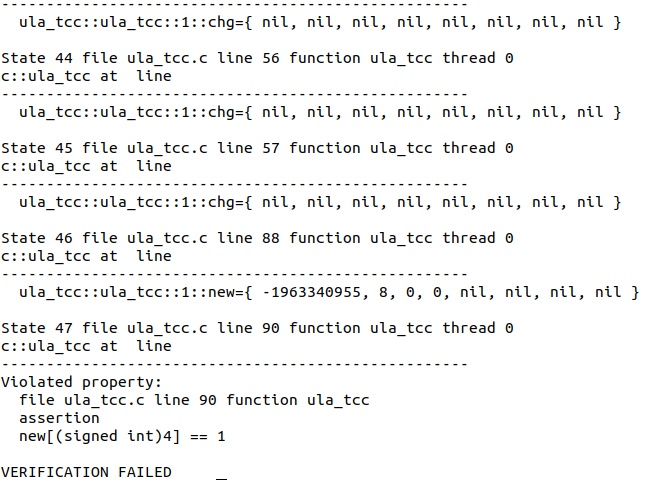
\includegraphics[scale=0.6]{Figuras/erro_assert.png}
	\end{center}
    \legend{Fonte:Própria}
\end{figure}